\documentclass[11pt]{article}
\usepackage[a4paper, total={6.8in, 9.25in}]{geometry}
\usepackage{graphicx}
\graphicspath{ {./assets/images/output/} }
\usepackage{caption}
\usepackage[english]{babel}
\usepackage{titling}
\usepackage{float}
\usepackage{amsmath}
\usepackage{algorithm}
\usepackage{algorithmicx}
\usepackage{algpseudocode}
\usepackage{minted}
\usepackage{multicol}
\usepackage{array}
\usepackage{setspace}
\usepackage{placeins}
\usepackage{tcolorbox}
\usepackage{caption}
\usepackage{subcaption}

\definecolor{verbgray}{gray}{.95}
\setminted{
    bgcolor=verbgray,
    baselinestretch=1,
    fontsize=\footnotesize,
    linenos,
    breaklines=true,
    breakanywhere=true,
    xleftmargin=\parindent
}
\title{Optimization of Neural Network Parameters Using Genetic Algorithms (Neuro-Genetic Approach)}
\author{}
\date{}

\pagenumbering{gobble}
\begin{document}
\input{ml_cover.tex}

\pagebreak

\tableofcontents

\pagebreak
\pagenumbering{arabic}
\maketitle

\section{Theory and Introduction}
Traditional Artificial Neural Networks (ANNs) rely on gradient-based optimization methods, such as Backpropagation and Gradient Descent, to update network weights and biases. While effective, gradient-based methods are prone to becoming trapped in local minima and require the activation functions to be strictly differentiable \cite{goodfellow2016deep}.

This experiment explores a derivative-free alternative: the **Neuro-Genetic Algorithm**. By framing the neural network parameters as a biological genome, Genetic Algorithms (GA) use evolutionary principles—Selection, Crossover, and Mutation—to iteratively optimize the network's weights.

\subsection{Chromosome Encoding}
To apply a genetic algorithm, the entire set of parameters for a given neural network must be encoded into a 1-dimensional array, known as a chromosome. For a network with weight matrices $W^{[1]}, W^{[2]}$ and bias vectors $b^{[1]}, b^{[2]}$, the chromosome $C$ is a flattened concatenation:
\begin{equation}
    C = \left[ \text{flatten}(W^{[1]}), \text{flatten}(b^{[1]}), \text{flatten}(W^{[2]}), \text{flatten}(b^{[2]}) \right]
\end{equation}

\subsection{Fitness Function}
The fitness function evaluates how well a specific chromosome solves the classification problem. Instead of minimizing a cost function, the GA maximizes fitness. The fitness $F$ is calculated using the inverse of the Binary Cross-Entropy (Log Loss) $J(C)$:
\begin{equation}
    J(C) = -\frac{1}{m} \sum_{i=1}^{m} \left[ y^{(i)} \log(\hat{y}^{(i)}) + (1 - y^{(i)}) \log(1 - \hat{y}^{(i)}) \right]
\end{equation}
\begin{equation}
    F(C) = \frac{1}{1 + J(C)}
\end{equation}
A lower loss yields a fitness closer to 1.0, while a higher loss yields a fitness closer to 0.

\subsection{Evolutionary Operators}
\begin{itemize}
    \item \textbf{Tournament Selection:} A subset of individuals is randomly selected, and the one with the highest fitness is chosen to be a parent.
    \item \textbf{Uniform Crossover:} Two parent chromosomes exchange genes (weights) to produce offspring. A random binary mask dictates which parent contributes which gene.
    \item \textbf{Gaussian Mutation:} Random noise is injected into the genes of the offspring to maintain genetic diversity and explore new regions of the parameter space:
          \begin{equation}
              C'_{mutated} = C' + \mathcal{N}(0, \sigma^2) \quad \text{(for genes selected by mutation rate)}
          \end{equation}
\end{itemize}

\section{Methodology}

\subsection{Dataset}
The synthetic \textit{Two Moons} dataset was utilized to evaluate the model's capacity to resolve non-linear classification problems. The dataset was standardized and split into 80\% training and 20\% testing sets.

\subsection{Algorithms}

\begin{algorithm}[H]
    \caption{Neuro-Genetic Optimization}
    \begin{algorithmic}[1]
        \State \textbf{Input:} Training Data $(X, Y)$, Population Size $N$, Generations $G$, Mutation Rate $\mu$
        \State \textbf{Initialize Population:} Generate $N$ random chromosomes (weight arrays)
        \For{$g = 1$ to $G$}
        \For{each chromosome $C_i$ in Population}
        \State Decode $C_i$ into $W^{[1]}, b^{[1]}, W^{[2]}, b^{[2]}$
        \State $\hat{Y} \gets \text{ForwardPass}(X, C_i)$
        \State $Fitness(C_i) \gets \frac{1}{1 + \text{LogLoss}(Y, \hat{Y})}$
        \EndFor
        \State \textbf{Elitism:} Keep the best performing chromosome
        \State $NewPopulation \gets [BestChromosome]$
        \While{size of $NewPopulation < N$}
        \State $P_1, P_2 \gets \text{TournamentSelection}(Population, Fitness)$
        \State $Child \gets \text{UniformCrossover}(P_1, P_2)$
        \State $MutatedChild \gets \text{GaussianMutation}(Child, \mu)$
        \State Append $MutatedChild$ to $NewPopulation$
        \EndWhile
        \State $Population \gets NewPopulation$
        \EndFor
        \State \Return $BestChromosome$
    \end{algorithmic}
\end{algorithm}

\subsection{Code}
The algorithm was implemented natively in Python. The neural network architecture utilized 2 input neurons, 5 hidden neurons (with Tanh activation), and 1 output neuron (with Sigmoid activation), resulting in a chromosome length of 21 genes.

\begin{multicols}{2}
    \inputminted{python}{./assets/neuro_genetic.py}
\end{multicols}

\section{Results and Discussion}
The Neuro-Genetic model was evolved over 150 generations with a population of 60 individuals. The performance progressively improved as favorable weights were selected and combined.

\subsection{Quantitative Results}
The console output logs demonstrate a steady increase in both the Best Fitness and Average Fitness of the population:

\begin{minted}{console}
==================================================
 NEURO-GENETIC OPTIMIZATION ALGORITHM
==================================================
Generating 'Two Moons' dataset...
Starting Genetic Evolution of Neural Network Parameters...
Initializing Population (60 individuals)...
Generation   0 | Best Fitness: 0.7992 | Avg Fitness: 0.5208
Generation  20 | Best Fitness: 0.8614 | Avg Fitness: 0.8194
Generation  40 | Best Fitness: 0.9131 | Avg Fitness: 0.8764
Generation  60 | Best Fitness: 0.9380 | Avg Fitness: 0.8982
Generation  80 | Best Fitness: 0.9457 | Avg Fitness: 0.9211
Generation 100 | Best Fitness: 0.9493 | Avg Fitness: 0.9168
Generation 120 | Best Fitness: 0.9516 | Avg Fitness: 0.9352
Generation 140 | Best Fitness: 0.9527 | Avg Fitness: 0.9362
Generation 149 | Best Fitness: 0.9531 | Avg Fitness: 0.9316
========================================
EVALUATION REPORT (Test Set)
========================================
Accuracy:  0.9667
Precision: 0.9636
Recall:    0.9636
F1 Score:  0.9636
Confusion Matrix:
[[63  2]
 [ 2 53]]
\end{minted}

The evaluation on the unseen test set yielded an excellent accuracy and F1 score of 96.67\% and 0.9636, respectively. The confusion matrix (Figure \ref{fig:nga_results}c) confirms an evenly balanced error rate, with exactly 2 false positives and 2 false negatives.

\subsection{Visual Analysis}

\begin{figure}[H]
    \centering
    \begin{subfigure}[b]{0.48\textwidth}
        \centering
        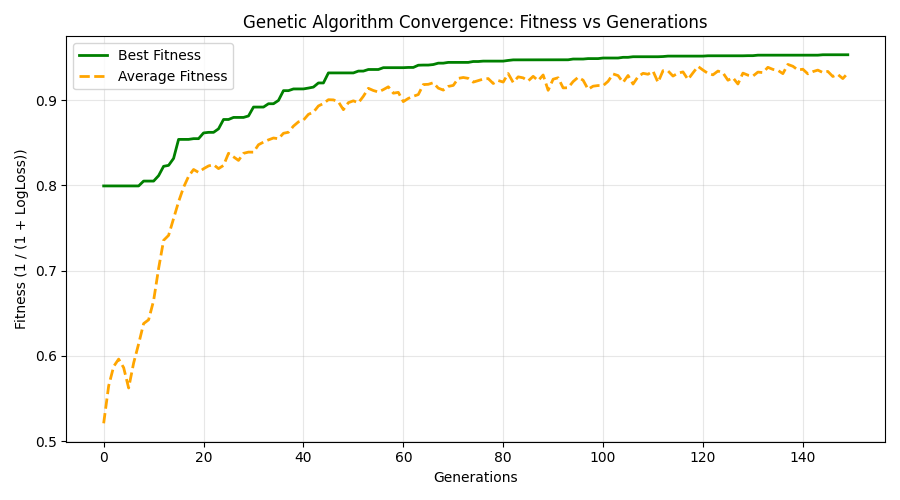
\includegraphics[width=\textwidth]{fitness_vs_gen.png}
        \caption{Fitness Convergence vs. Generations}
    \end{subfigure}
    \hfill
    \begin{subfigure}[b]{0.48\textwidth}
        \centering
        
\includegraphics[width=\textwidth]{decision.png}
        \caption{Evolved Non-Linear Decision Boundary}
    \end{subfigure}

    \vspace{0.5cm}
    \begin{subfigure}[b]{0.5\textwidth}
        \centering
        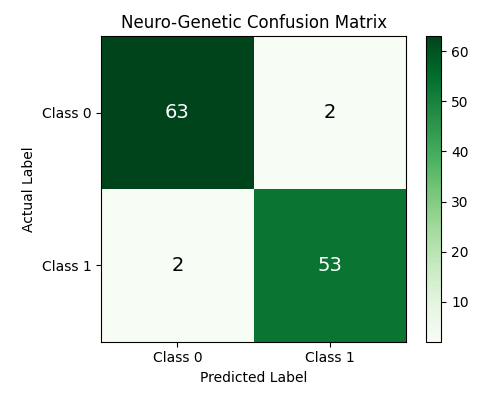
\includegraphics[width=0.7\textwidth]{conf.png}
        \caption{Neuro-Genetic Confusion Matrix}
    \end{subfigure}
    \caption{Neuro-Genetic Algorithm Performance Overview}
    \label{fig:nga_results}
\end{figure}

\begin{itemize}
    \item \textbf{Fitness Convergence (Figure \ref{fig:nga_results}a):} The convergence plot illustrates classic evolutionary behavior. The \textit{Best Fitness} (solid green line) acts as an upper bound that incrementally steps up whenever a favorable mutation or crossover is discovered. The \textit{Average Fitness} (dashed orange line) closely follows it, indicating that the overall genetic quality of the population rapidly stabilizes and improves over time.
    \item \textbf{Decision Boundary (Figure \ref{fig:nga_results}b):} The resulting neural network was able to map a highly non-linear boundary that accurately traces the "Two Moons" geometric distribution. This proves that a derivative-free GA approach can successfully navigate a complex, 21-dimensional parameter space to find an optimal solution.
\end{itemize}

\section{Conclusion}
This experiment successfully demonstrated the viability of the Neuro-Genetic approach for training Artificial Neural Networks. By discarding traditional gradient descent in favor of evolutionary principles, the algorithm effectively optimized the network weights and achieved an accuracy of 96.67\% on a complex non-linear dataset. While computationally expensive due to evaluating entire populations per generation, Genetic Algorithms provide a robust alternative for non-differentiable network architectures and complex loss landscapes where gradient methods might fail.

\bibliographystyle{IEEEtran}
\renewcommand{\bibname}{References}
\addcontentsline{toc}{section}{References}
\bibliography{ref}

\end{document}